% Plantilla original de Beamer: https://www.overleaf.com
\documentclass{beamer}

\usetheme{Madrid}
\usecolortheme{default}
\usefonttheme{serif}
\setbeamertemplate{navigation symbols}{}
\setbeamertemplate{caption}[numbered]

\usepackage[spanish]{babel}
\usepackage[T1]{fontenc}

% Recursos para las diapositivas.
\usepackage{graphicx}
\usepackage{amsmath,amssymb}
\usepackage{booktabs}
\usepackage{siunitx}
\usepackage{tikz}
\usetikzlibrary{arrows.meta,positioning}
\usepackage{listings}

\graphicspath{{Informe_19_11_2026/attachments/}}
\sisetup{output-decimal-marker={,}}

% Cambiar a \ejemplostrue para ver los ejemplos al final del PDF.
\newif\ifejemplos
\ejemplosfalse

% Descomentar para generar una versión con notas del orador.
% \setbeameroption{show notes}

% Cambiar a \referenciastrue una vez que se incorporen citas.
% Compilar con latexmk -pdf presentacion.tex desde la carpeta Informe.
\newif\ifreferencias
\referenciasfalse


\title[Control de un brazo con PMSM]{Control de accionamiento de CA con motor sincrónico de imanes permanentes}
\subtitle{Proyecto Global Integrador de Automática y Máquinas Eléctricas}
\author[Barrios y Muñiz]{Federico Barrios R. \and Lucia Muñiz}
\institute[UNCuyo]{Ingeniería Mecatrónica\\Facultad de Ingeniería, Universidad Nacional de Cuyo}
\date{} % Completar con la fecha de exposición.

\begin{document}

\begin{frame}
  \titlepage
\end{frame}

\begin{frame}[t]{Contenidos}
  \small
  \begin{columns}[T,onlytextwidth]
    \begin{column}{0.49\textwidth}
      \begin{enumerate}
        \item \textbf{Introducción}
          \begin{enumerate}
            \item Sistemas considerados
            \item Actuadores
            \item Sensores
            \item Espacio de Park
          \end{enumerate}
        \item \textbf{Modelado, análisis y simulación dinámica a lazo abierto}
          \begin{enumerate}
            \item Sistema mecánico equivalente
            \item Modelo global no lineal
            \item Linealización
            \item Análisis de estabilidad a lazo abierto, controlabilidad y observabilidad
            \item Simulaciones dinámicas
          \end{enumerate}
      \end{enumerate}
    \end{column}
    \begin{column}{0.49\textwidth}
      \begin{enumerate}
        \setcounter{enumi}{2}
        \item \textbf{Diseño, análisis y simulación con controlador de movimiento en cascada con modulador de torque equivalente}
          \begin{enumerate}
            \item Modulador de torque equivalente
            \item Controlador de movimiento
            \item Observador de estado
            \item Simulación en tiempo continuo
            \item Verificación de desempeño y/o mejoras
            \item Versión final y discretización
          \end{enumerate}
        \item \textbf{Conclusiones}
      \end{enumerate}
    \end{column}
  \end{columns}
\end{frame}

\section{Introducción}

\begin{frame}{Sistemas considerados}
  \begin{itemize}
    \item Brazo con eje horizontal, transmisión reductora y motor PMSM.
    \item Seguimiento de la posición angular para las cargas especificadas.
    \item Límites de tensión, corriente y temperatura del accionamiento.
  \end{itemize}
  % Agregar el esquema del brazo y la consigna original del enunciado.
\end{frame}

\begin{frame}{Actuadores}
  \begin{itemize}
    \item Motor sincrónico de imanes permanentes (PMSM).
    \item Inversor trifásico de alimentación del estator.
  \end{itemize}
  % Agregar el esquema del accionamiento y los datos nominales.
\end{frame}

\begin{frame}{Sensores}
  \begin{itemize}
    \item Codificador incremental para medir la posición angular del motor.
    \item Sensores de corriente en las tres fases del estator.
    \item Sensor de temperatura en el bobinado del estator.
  \end{itemize}
\end{frame}

\begin{frame}{Espacio de Park}
  \begin{itemize}
    \item Transformación de las variables trifásicas al marco $dq0$ ligado al rotor.
    \item Ejes directo, en cuadratura y homopolar.
  \end{itemize}
  % Agregar el esquema de los ejes y la transformación utilizada.
\end{frame}

\section[Modelado a lazo abierto]{Modelado, análisis y simulación dinámica a lazo abierto}

\begin{frame}{Sistema mecánico equivalente}
  \begin{itemize}
    \item Dinámica de la carga y la transmisión referida al eje del motor.
    \item Inercia equivalente, fricción y torque gravitatorio.
  \end{itemize}
  % Agregar el balance de torques referido al eje del motor.
\end{frame}

\begin{frame}{Modelo global no lineal}
  \begin{itemize}
    \item Acoplamiento de los subsistemas mecánico, electromagnético y térmico.
    \item Modelo electromagnético en los ejes de Park.
    \item Comportamiento térmico del estator y variación de su resistencia.
  \end{itemize}
  % Agregar el diagrama de bloques del modelo global no lineal.
\end{frame}

\begin{frame}{Linealización}
  \begin{itemize}
    \item Modelo LPV obtenido por linealización jacobiana.
    \item Modelo LTI equivalente aumentado a partir del desacoplamiento por realimentación no lineal y las hipótesis de simplificación.
  \end{itemize}
  % Resumir las hipótesis de cada modelo.
\end{frame}

\begin{frame}{Análisis de estabilidad a lazo abierto, controlabilidad y observabilidad}
  \begin{itemize}
    \item Polos de la planta y efecto de la perturbación de carga.
    \item Controlabilidad del subsistema de movimiento desde la tensión en cuadratura.
    \item Observabilidad desde la posición y alcance de la medición de velocidad.
  \end{itemize}
  % Agregar el mapa de polos y ceros. Explicitar qué subsistema se analiza.
\end{frame}

\begin{frame}{Simulaciones dinámicas}
  \begin{itemize}
    \item Comparación de las respuestas del modelo no lineal desacoplado y del modelo LTI.
  \end{itemize}
  % Mostrar un transitorio y las condiciones del ensayo.
\end{frame}

\section[Control de movimiento en cascada]{Diseño, análisis y simulación con controlador de movimiento en cascada con modulador de torque equivalente}

\begin{frame}{Modulador de torque equivalente}
  \begin{itemize}
    \item Compensación de los torques de gravedad y fricción.
    \item Lazos internos de corriente y modulación de tensión para compensar los acoplamientos eléctricos.
  \end{itemize}
  % Agregar el diagrama del modulador e identificar sus entradas y salidas.
\end{frame}

\begin{frame}{Controlador de movimiento}
  \begin{itemize}
    \item Lazo externo de movimiento y selección de ganancias del PID por asignación de polos.
    \item Coordinación de los tiempos de respuesta del lazo de movimiento y los lazos de corriente.
  \end{itemize}
  % Mostrar los polos elegidos y la ubicación del PID en el diagrama global.
\end{frame}

\begin{frame}{Observador de estado}
  \begin{itemize}
    \item Estimador de orden reducido para reconstruir la velocidad angular a partir de la posición medida.
  \end{itemize}
  % Agregar una comparación de la velocidad del modelo y la velocidad estimada.
\end{frame}

\begin{frame}{Simulación en tiempo continuo}
  \begin{itemize}
    \item Exigencias de aceleración, corriente y tensión de la consigna original.
    \item Suavizado de las transiciones y seguimiento con las cargas ensayadas.
    \item Respuesta ante perturbaciones de carga.
  \end{itemize}
  % Agregar la comparación de perfiles y una curva de seguimiento.
\end{frame}

\begin{frame}{Verificación de desempeño y/o mejoras}
  \begin{itemize}
    \item Evolución de la temperatura del estator y comparación con el límite de operación del motor.
    \item Efecto del ancho de banda finito de los sensores y del inversor, y de la saturación de tensión.
    \item Comparación de las respuestas con parámetros nominales y con el ancho de banda modificado.
  \end{itemize}
  % Agregar la curva térmica y un ensayo comparativo con componentes no ideales.
\end{frame}

\begin{frame}{Versión final y discretización}
  \begin{itemize}
    \item Selección del período de muestreo y discretización del PID y del estimador.
    \item Implementación con bloques de Simulink y en \texttt{MATLAB Function}.
  \end{itemize}
  % Agregar el esquema discreto y el resultado de simulación que se usará en la demostración.
\end{frame}

\section{Conclusiones}

\begin{frame}{Conclusiones}
  \begin{itemize}
    \item El modelo LTI orientó el diseño del control en cascada, que se evaluó sobre la planta no lineal.
    \item El suavizado de la consigna permitió seguir la posición en simulación para las cargas ensayadas.
    \item La temperatura del estator y el ancho de banda de los equipos condicionan el desempeño del accionamiento.
  \end{itemize}
\end{frame}

% Si hay citas en la presentación, activar \referenciastrue en el preámbulo.
% Claves disponibles: julian2026guia, krause2013electric,
% astrom2020feedback y ogata2010control.
\ifreferencias
\begin{frame}[allowframebreaks]{Referencias}
  \bibliographystyle{plain}
  \bibliography{Informe_19_11_2026/references}
\end{frame}
\fi

% Herramientas reutilizables. Copiar los frames necesarios al cuerpo.
% En las figuras, usar \linewidth para respetar el ancho de la columna.
\ifejemplos
\appendix

% Bloques de Beamer. Copiar el entorno que se necesite dentro de un frame.
% block, alertblock y exampleblock reciben un título entre llaves.
% theorem, lemma, corollary, definition, example y proof admiten un título
% opcional entre corchetes.
% Para crear un entorno propio, agregar al preámbulo, por ejemplo:
% \newtheorem{proposicion}{Proposición}

\begin{frame}{Bloques de texto}
  \begin{block}{Hipótesis del modelo}
    El brazo gira alrededor de un eje horizontal fijo.
  \end{block}

  \begin{alertblock}{Restricción del accionamiento}
    La tensión aplicada al estator está limitada por el inversor.
  \end{alertblock}

  \begin{exampleblock}{Caso de simulación}
    Comparar las consignas original y suavizada para la misma carga.
  \end{exampleblock}
\end{frame}

\begin{frame}{Teorema y demostración}
  \begin{theorem}[Estabilidad de un sistema de primer orden]
    Si $a>0$, el origen de $\dot{x}=-ax$ es exponencialmente estable.
  \end{theorem}

  \begin{proof}
    La solución es $x(t)=x(0)e^{-at}$. Por lo tanto,
    $\lvert x(t)\rvert=e^{-at}\lvert x(0)\rvert$ para todo $t\geq 0$.
  \end{proof}
\end{frame}

\begin{frame}{Definición y ejemplo}
  \begin{definition}[Error de seguimiento]
    El error de posición es $e_\theta(t)=\theta^\ast(t)-\theta(t)$,
    donde $\theta^\ast$ es la consigna y $\theta$ es la posición medida.
  \end{definition}

  \begin{example}
    Si $\theta^\ast=\qty{1}{\radian}$ y $\theta=\qty{0.9}{\radian}$,
    entonces $e_\theta=\qty{0.1}{\radian}$.
  \end{example}
\end{frame}

\begin{frame}{Lema y corolario}
  \begin{lemma}[Transmisión rígida]
    Para una relación de transmisión constante $r>0$, si
    $\theta_l=\theta_m/r$, entonces $\omega_l=\omega_m/r$.
  \end{lemma}

  \begin{corollary}
    Si el eje del motor permanece en reposo, la carga también permanece
    en reposo bajo la hipótesis de transmisión rígida.
  \end{corollary}
\end{frame}

\begin{frame}[t]{Figura y texto en columnas}
  \begin{columns}[T,onlytextwidth]
    \begin{column}{0.48\textwidth}
      \begin{figure}
        \centering
        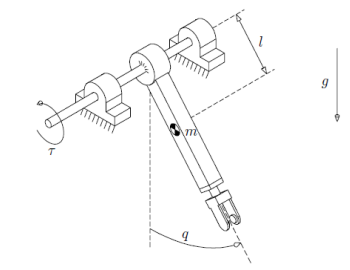
\includegraphics[width=\linewidth,height=0.52\textheight,keepaspectratio]
          {Esquema de la carga.png}
        \caption{Esquema de la carga.}
        \label{fig:ejemplo-carga}
      \end{figure}
    \end{column}
    \begin{column}{0.47\textwidth}
      La Figura~\ref{fig:ejemplo-carga} muestra el brazo y su eje de giro.
    \end{column}
  \end{columns}
\end{frame}

\begin{frame}{Diagrama en PDF}
  \centering
  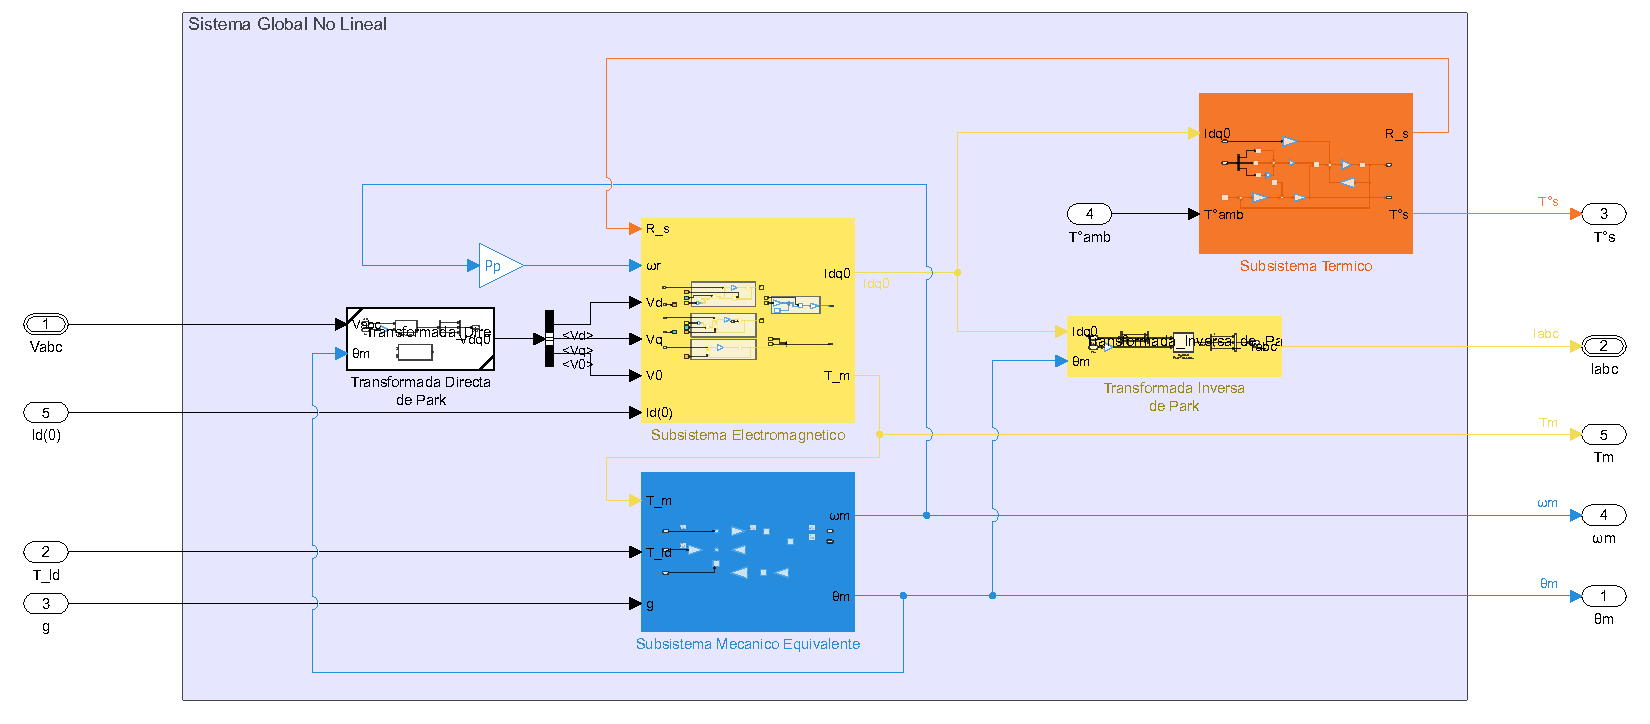
\includegraphics[width=\linewidth,height=0.72\textheight,keepaspectratio]
    {Bloque Modelo Global No Lineal.pdf}
\end{frame}

\begin{frame}{Comparación de dos gráficas}
  \begin{columns}[T,onlytextwidth]
    \begin{column}{0.48\textwidth}
      \centering
      \textbf{Consigna original}\par\smallskip
      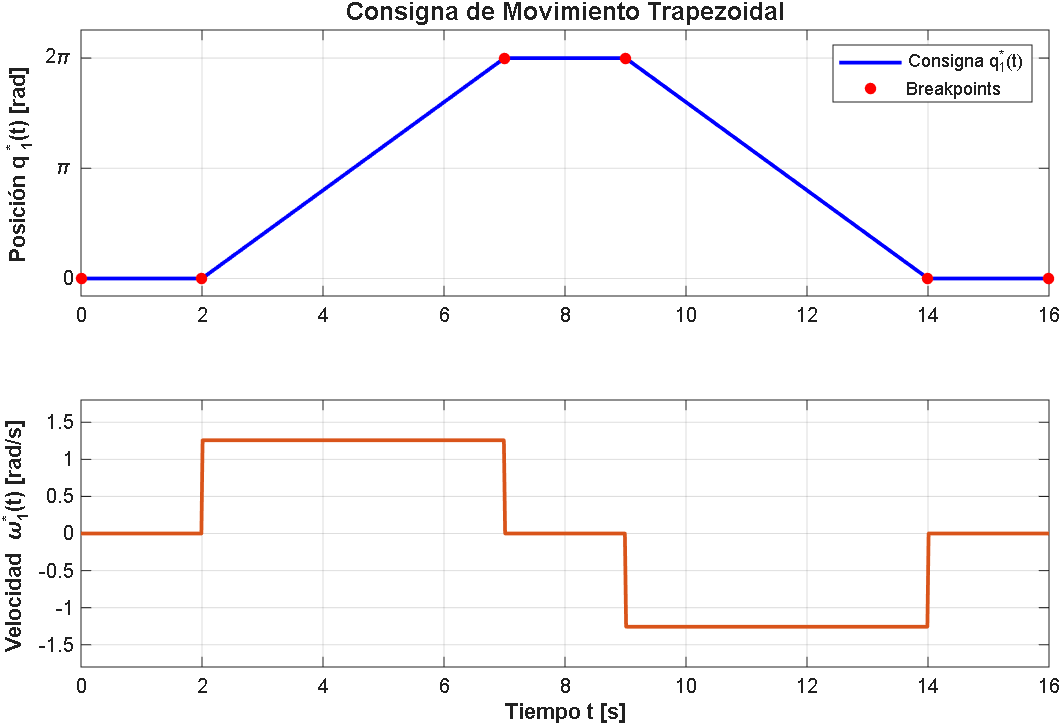
\includegraphics[width=\linewidth,height=0.56\textheight,keepaspectratio]
        {consigna movimiento posición.png}
    \end{column}
    \begin{column}{0.48\textwidth}
      \centering
      \textbf{Consigna suavizada}\par\smallskip
      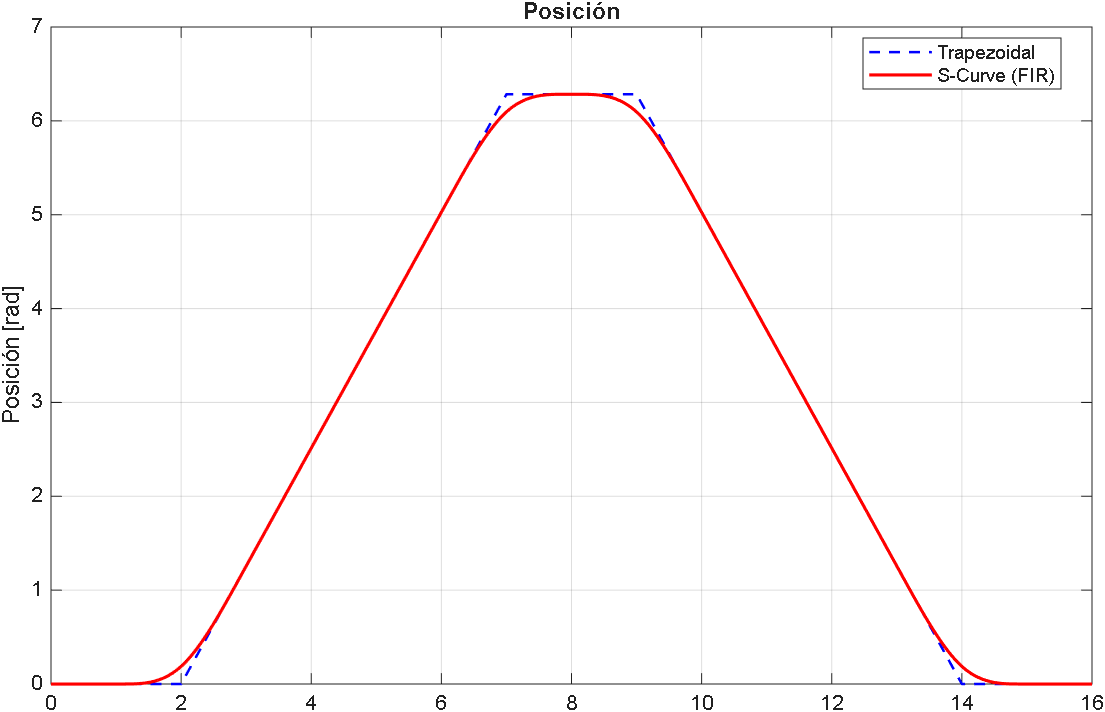
\includegraphics[width=\linewidth,height=0.56\textheight,keepaspectratio]
        {Consigna de movimiento suavizada.png}
    \end{column}
  \end{columns}
\end{frame}

\begin{frame}{Ecuaciones y referencias cruzadas}
  \begin{align}
    \Delta\dot{\mathbf{x}} &= A\Delta\mathbf{x} + B\Delta\mathbf{u},
      \label{eq:ejemplo-estado}\\
    \Delta\mathbf{y} &= C\Delta\mathbf{x} + D\Delta\mathbf{u}.
  \end{align}
  La ecuación~\eqref{eq:ejemplo-estado} describe la dinámica del estado.
  % Para ecuaciones sin numerar, usar align* o \[ ... \].
\end{frame}

\begin{frame}{Tabla y unidades}
  \centering
  \begin{tabular}{@{}ll@{}}
    \toprule
    Variable & Unidad \\
    \midrule
    Posición angular & \unit{\radian} \\
    Velocidad angular & \unit{\radian\per\second} \\
    Torque & \unit{\newton\metre} \\
    Temperatura & \unit{\degreeCelsius} \\
    \bottomrule
  \end{tabular}

  % Ejemplo de valor con unidad: \qty{0.1}{\second}.
  % Para alinear números por el separador decimal, usar columnas S de siunitx.
\end{frame}

\begin{frame}{Diagrama de bloques editable}
  \centering
  \begin{tikzpicture}[
      node distance=6mm,
      bloque/.style={draw, align=center, minimum height=8mm},
      >={Latex}
    ]
    \node (ref) {$\theta^\ast$};
    \node[bloque,right=of ref] (pid) {PID};
    \node[bloque,right=of pid] (mod) {Modulador\\de torque};
    \node[bloque,right=of mod] (planta) {Planta};
    \node[right=of planta] (pos) {$\theta$};
    \draw[->] (ref) -- (pid);
    \draw[->] (pid) -- (mod);
    \draw[->] (mod) -- (planta);
    \draw[->] (planta) -- (pos);
    \draw[->] (pos.south) -- ++(0,-8mm) -| (pid.south);
  \end{tikzpicture}
\end{frame}

\begin{frame}[fragile]{Fragmento de código MATLAB}
  % Mantener [fragile] para que Beamer pueda leer el entorno lstlisting.
  \begin{lstlisting}[language=Matlab,basicstyle=\ttfamily\small,columns=fullflexible,breaklines=true]
e_pos = theta_ref - theta;
e_vel = omega_ref - omega_est;
u = Kp * e_pos + Kd * e_vel + Ki * integral_e;
  \end{lstlisting}
\end{frame}

\begin{frame}[label=ejemplo-exposicion]{Aparición progresiva y notas}
  % Quitar [<+->] si se quieren mostrar todos los puntos desde el inicio.
  \begin{enumerate}[<+->]
    \item Presentar la consigna y las condiciones del ensayo.
    \item Comparar el seguimiento con las restricciones del equipo.
    \item Destacar con \alert{una frase} el resultado del ensayo.
  \end{enumerate}
  \note{Mencionar qué masa se simuló y qué variables se usaron para comparar los casos.}
\end{frame}

\begin{frame}{Enlaces y citas}
  \hyperlink{ejemplo-exposicion}{\beamerbutton{Volver al ejemplo anterior}}

  \medskip
  \href{https://www.uncuyo.edu.ar/}{Universidad Nacional de Cuyo}

  \medskip
  \ifreferencias
    Transformación de Park y modelado de máquinas eléctricas~\cite{krause2013electric}.
  \else
    % Activar \referenciastrue para mostrar en esta diapositiva el ejemplo de \cite.
    Comando de ejemplo: \texttt{\textbackslash cite\{krause2013electric\}}.
  \fi
\end{frame}
\fi

\end{document}
